\documentclass{article}
\usepackage{fontspec}
\usepackage{float}
\usepackage[left=2.5cm,right=2cm,top=2cm,bottom=2.5cm]{geometry} 
\setlength{\parindent}{0pt}
\usepackage{graphicx} 
\graphicspath{{images/}{./}}
\usepackage[table]{xcolor}
\usepackage{longtable}
\usepackage{tikz}
\usetikzlibrary{arrows.meta, shapes.geometric, arrows, positioning, calc, matrix, fit}
\usepackage{pgfplots}
\pgfplotsset{compat=1.18}
\usepackage{scrextend}
\changefontsizes{13pt}
\usepackage{fancyvrb}
\usepackage{array}
\usepackage{multirow}
\usepackage{framed}
\usepackage{amsmath}
\usepackage{amsfonts}
\usepackage{amssymb}
\usepackage{setspace}
\usepackage{booktabs}
\usepackage{tabularx}
\usepackage[ruled,vlined,linesnumbered]{algorithm2e}
\usepackage{enumitem}
\usepackage[hidelinks]{hyperref}
\definecolor{primarycolor}{RGB}{10, 50, 180}
\definecolor{solved}{RGB}{18, 128, 91}
\definecolor{stuck}{RGB}{180, 110, 0}
\definecolor{incons}{RGB}{196, 49, 58}
\definecolor{filterc}{RGB}{79, 70, 229}
\definecolor{naivec}{RGB}{236, 160, 60}
\definecolor{counterc}{RGB}{20, 150, 120}
\usepackage{sectsty}
\sectionfont{\color{primarycolor}}
\subsectionfont{\color{primarycolor}}
\renewcommand{\tablename}{Bảng}
\renewcommand{\figurename}{Hình}
\renewcommand{\contentsname}{Mục lục}
\renewcommand{\algorithmcfname}{Thuật toán}
\setstretch{1.25}
\emergencystretch=2em
\fvset{fontsize=\small, frame=single, framesep=6pt, rulecolor=\color{gray!50}}

\newcommand{\code}[1]{\texttt{#1}}
\newcommand{\KB}{\mathit{KB}}

\begin{document}

% --- TRANG BÌA ---
\hypersetup{pageanchor=false}
\begin{titlepage}
\begin{tikzpicture}[remember picture,overlay,inner sep=0,outer sep=0]
     \draw[blue!70!black,line width=4pt] ([xshift=-1.5cm,yshift=-2cm]current page.north east) coordinate (A)--([xshift=1.5cm,yshift=-2cm]current page.north west) coordinate(B)--([xshift=1.5cm,yshift=2cm]current page.south west) coordinate (C)--([xshift=-1.5cm,yshift=2cm]current page.south east) coordinate(D)--cycle;

     \draw ([yshift=0.5cm,xshift=-0.5cm]A)-- ([yshift=0.5cm,xshift=0.5cm]B)--
     ([yshift=-0.5cm,xshift=0.5cm]B) --([yshift=-0.5cm,xshift=-0.5cm]B)--([yshift=0.5cm,xshift=-0.5cm]C)--([yshift=0.5cm,xshift=0.5cm]C)--([yshift=-0.5cm,xshift=0.5cm]C)-- ([yshift=-0.5cm,xshift=-0.5cm]D)--([yshift=0.5cm,xshift=-0.5cm]D)--([yshift=0.5cm,xshift=0.5cm]D)--([yshift=-0.5cm,xshift=0.5cm]A)--([yshift=-0.5cm,xshift=-0.5cm]A)--([yshift=0.5cm,xshift=-0.5cm]A);

     \draw ([yshift=-0.3cm,xshift=0.3cm]A)-- ([yshift=-0.3cm,xshift=-0.3cm]B)--
     ([yshift=0.3cm,xshift=-0.3cm]B) --([yshift=0.3cm,xshift=0.3cm]B)--([yshift=-0.3cm,xshift=0.3cm]C)--([yshift=-0.3cm,xshift=-0.3cm]C)--([yshift=0.3cm,xshift=-0.3cm]C)-- ([yshift=0.3cm,xshift=0.3cm]D)--([yshift=-0.3cm,xshift=0.3cm]D)--([yshift=-0.3cm,xshift=-0.3cm]D)--([yshift=0.3cm,xshift=-0.3cm]A)--([yshift=0.3cm,xshift=0.3cm]A)--([yshift=-0.3cm,xshift=0.3cm]A);
\end{tikzpicture}
   
\begin{center}
    \vspace{7pt}
    \textbf{ĐẠI HỌC QUỐC GIA THÀNH PHỐ HỒ CHÍ MINH} \\
    \textbf{TRƯỜNG ĐẠI HỌC KHOA HỌC TỰ NHIÊN}
\end{center}

\vspace{1pt}
\begin{center}
    
\includegraphics[width=3.5cm]{hcmus.png}
    
    \vspace{15pt}
    \fontsize{18pt}{17pt}\selectfont
    \textbf{Báo cáo Đồ án} \\
    \textbf{Cơ sở Trí tuệ nhân tạo} \\
\end{center}

\begin{flushleft}
    \fontsize{15pt}{13pt}\selectfont
    \textbf{\textsl{Project 2}}
\end{flushleft}

\begin{center}
    {\fontsize{24pt}{28pt}\selectfont\textbf{\textcolor{primarycolor}{GRIDUCTIVE SOLVER}}}
\end{center}

\begin{flushright}
\begin{center}
    \textbf{Nhóm thực hiện:}
    \vspace{1pt}
    
    \renewcommand{\arraystretch}{1.3}
    {\small
    \begin{tabular}{l @{\hspace{1.5cm}} l} 
        \textit{\small Họ và tên} & \textit{\small MSSV} \\
        \textbf{Trần Quốc Khanh}    & \textbf{24122001} \\
        \textbf{Lê Gia Khánh}       & \textbf{24122005} \\
        \textbf{Trần Trung Hiếu}    & \textbf{24122033} \\
        \textbf{Phạm Chấn Khoa}     & \textbf{24122038} \\
        \textbf{Cái Hoàng Bảo Kin}  & \textbf{24122040} \\
    \end{tabular}
    }
\end{center}
\end{flushright}
\end{titlepage}
\hypersetup{pageanchor=true}

% --- MỤC LỤC ---
\tableofcontents
\newpage

% =========================================================================
% CHƯƠNG 1: KẾ HOẠCH & PHÂN CÔNG
% =========================================================================
\section{Kế hoạch thực hiện \& Phân công công việc}

\subsection{Kế hoạch \& Tiến độ triển khai}
Dự án được triển khai trong 3 tuần với các mốc chính:
\begin{itemize}[noitemsep]
    \item \textbf{Tuần 1:} Nghiên cứu luật chơi Griductive và logic mệnh đề; xây dựng mô hình lưới, ngôn ngữ manh mối và bộ đánh giá ngữ nghĩa trực tiếp; tự cài đặt bộ giải SAT DPLL kèm bộ kiểm thử đối chiếu vét cạn.
    \item \textbf{Tuần 2:} Bộ mã hóa CNF tự động cho 6 mẫu manh mối cốt lõi và các phần mở rộng (mã hóa tổ hợp trực tiếp và bộ đếm tuần tự Tseitin); tách \code{GameEngine} và \code{LogicAgent}; phân loại hệ quả logic, vòng suy diễn không đoán, Hint, kiểm tra nghiệm duy nhất; bộ sinh câu đố.
    \item \textbf{Tuần 3:} Giao diện web \textit{Casebook} (máy chủ HTTP dùng thư viện chuẩn, giao diện HTML, CSS và JavaScript), bộ nhân vật cầu thủ kèm ảnh chân dung, luật \textit{game over}; chạy thực nghiệm, review chéo nhiều vòng. Song song, nhóm báo cáo viết báo cáo, lên kịch bản video; quay và biên tập video demo.
\end{itemize}

\subsection{Phân công công việc chi tiết}
Nhóm chia thành hai mảng: ba thành viên phụ trách mã nguồn (Lê Gia Khánh, Trần Trung Hiếu, Phạm Chấn Khoa), hai thành viên phụ trách báo cáo và video (Trần Quốc Khanh, Cái Hoàng Bảo Kin). Tất cả các thành viên đều hoàn thành khối lượng công việc được giao:

\begin{table}[H]
\centering
\small
\renewcommand{\arraystretch}{1.3}
\begin{tabularx}{\textwidth}{|c|l|>{\raggedright\arraybackslash}X|c|}
\hline
\rowcolor{gray!20}
\textbf{STT} & \textbf{Thành viên} & \textbf{Nhiệm vụ cụ thể} & \textbf{Đóng góp} \\
\hline
1 & \textbf{Lê Gia Khánh} & \textit{Lập trình:} kiến trúc tách \code{GameEngine}/\code{LogicAgent} (\code{engine.py}, \code{agent.py}, \code{knowledge.py}); phân loại hệ quả $\KB_t \models C_i$, chiến lược lọc mô hình, Hint tối thiểu và kiểm tra nghiệm duy nhất (\code{entailment.py}); vòng suy diễn, trace, luật \textit{game over}; định dạng và bộ sinh câu đố (\code{puzzle.py}, \code{generator.py}); quản lý kho GitHub, chuẩn hóa mã và chú thích. & 100\% \\
\hline
2 & \textbf{Trần Trung Hiếu} & \textit{Lập trình:} mô hình lưới và vùng (\code{board.py}); ngôn ngữ manh mối và bộ đánh giá ngữ nghĩa (\code{clues.py}); bộ mã hóa CNF, mã hóa tổ hợp và bộ đếm Tseitin (\code{cnf.py}); bộ giải DPLL (\code{dpll.py}); bộ kiểm thử đối chiếu vét cạn. \textit{Video:} quay video demo. & 100\% \\
\hline
3 & \textbf{Phạm Chấn Khoa} & \textit{Lập trình:} máy chủ JSON (\code{server.py}) và giao diện web \textit{Casebook} (\code{web/}): lật thẻ, đánh dấu manh mối, Hint, Step/Auto Solve, tab Trace/Solver, màn hình \textit{game over}; bộ nhân vật cầu thủ và ảnh chân dung (\code{themes.py}, \code{tools/add\_portrait.py}); chương trình thực nghiệm (\code{experiments.py}). & 100\% \\
\hline
4 & \textbf{Trần Quốc Khanh} & \textit{Báo cáo:} viết báo cáo LaTeX (mô hình hóa, dẫn xuất CNF, mô tả thuật toán), tổng hợp và phân tích kết quả thực nghiệm, tài liệu tham khảo và phụ lục. \textit{Video:} cùng lên kịch bản demo. & 100\% \\
\hline
5 & \textbf{Cái Hoàng Bảo Kin} & \textit{Báo cáo:} viết phần giao diện, kiểm thử và hướng dẫn chạy; trình bày hình ảnh, bảng biểu. \textit{Video:} lên kịch bản demo, biên tập (edit) video, thêm thuyết minh/phụ đề và đăng lên Google Drive. & 100\% \\
\hline
\end{tabularx}
\caption{Bảng phân công nhiệm vụ và mức độ hoàn thành của các thành viên.}
\label{tab:phan_cong_cong_viec}
\end{table}

% =========================================================================
% CHƯƠNG 2: MÔ HÌNH HÓA BÀI TOÁN
% =========================================================================
\section{Mô hình hóa bài toán}

\subsection{Luật chơi \& Biểu diễn biến logic}
\textbf{Griductive} là trò chơi suy luận trên lưới $N \times N$ ($N \in \{3,4,5\}$). Mỗi ô chứa một nhân vật có trạng thái bí mật là \textbf{Criminal} hoặc \textbf{Innocent}, cùng một manh mối có cấu trúc (có thể trống). Ô được ký hiệu cột--hàng (ví dụ \code{C2} là cột C, hàng 2); các nhân vật được xếp theo thứ tự bảng chữ cái của tên, theo hàng. Mọi manh mối đã lật đều đúng, bất kể người nói là ai.

Quy tắc cốt lõi là \textbf{không được đoán}: một phán đoán chỉ được chấp nhận khi nó là hệ quả logic của tri thức công khai hiện tại ($\KB_t \models C_i$ hoặc $\KB_t \models \neg C_i$). Khi phán đoán đúng, thẻ được lật và manh mối của thẻ được thêm vào $\KB_{t+1}$.

Với mỗi nhân vật tại ô $i$, ta định nghĩa một biến mệnh đề chính:
\begin{equation}
C_i =
\begin{cases}
\text{True}, & \text{nếu nhân vật } i \text{ là Criminal} \\
\text{False}, & \text{nếu nhân vật } i \text{ là Innocent}
\end{cases}
\end{equation}
Ánh xạ biến là tất định: ô có chỉ số $r$ (đếm từ 0) theo thứ tự hàng (\code{A1, B1, \dots, A2, \dots}) có số hiệu $r+1$, nên các biến chính là $1,\dots,N^2$. Vì tên nhân vật được xếp theo bảng chữ cái theo hàng, thứ tự này trùng với thứ tự tên. Các biến phụ do bộ mã hóa sinh ra được đánh số \textbf{sau} $N^2$, nên luôn tách biệt với biến chính (\code{CNF.num\_primary}, \code{CNF.num\_aux}).

\subsection{Ngữ nghĩa manh mối}
Với vùng $R$ và đối tượng đếm \textit{who}, đặt literal $\ell_i = C_i$ nếu đếm tội phạm và $\ell_i = \neg C_i$ nếu đếm người vô tội.

\begin{table}[H]
\centering\small
\renewcommand{\arraystretch}{1.25}
\begin{tabularx}{\textwidth}{l X l}
\toprule
\textbf{Manh mối} & \textbf{Ý nghĩa} & \textbf{Nội dung logic} \\
\midrule
\code{FACT}$(i,s)$ & Nhân vật $i$ có trạng thái $s$ & $C_i$ hoặc $\neg C_i$ \\
\code{SAME}$(i,j)$ & Hai người cùng trạng thái & $C_i \leftrightarrow C_j$ \\
\code{DIFFERENT}$(i,j)$ & Hai người khác trạng thái & $C_i \oplus C_j$ \\
\code{EXACTLY}$(k,R)$ & Đúng $k$ người trong $R$ & $\sum_{i\in R} \ell_i = k$ \\
\code{AT\_LEAST}$(k,R)$ & Ít nhất $k$ người trong $R$ & $\sum_{i\in R} \ell_i \ge k$ \\
\code{AT\_MOST}$(k,R)$ & Nhiều nhất $k$ người trong $R$ & $\sum_{i\in R} \ell_i \le k$ \\
\midrule
\textit{MR1} \code{PARITY}$(R)$ & Số người trong $R$ là chẵn/lẻ & $\ell_1 \oplus \dots \oplus \ell_n = 0/1$ \\
\textit{MR2} \code{COMPARE}$(R_1,R_2)$ & So sánh số người giữa hai vùng & $\sum_{R_1}\ell \;\{>,<,=\}\; \sum_{R_2}\ell$ \\
\textit{MR3} \code{CONNECTED}$(R)$ & Những người được đếm trên một đoạn thẳng nằm liền nhau & $\forall a<b<c:\ \ell_a \land \ell_c \to \ell_b$ \\
\textit{MR4} \code{IMPLIES}$(p,q)$ & Manh mối ghép ``nếu \dots\ thì \dots'' & $p \to q$ \\
\bottomrule
\end{tabularx}
\caption{6 mẫu manh mối cốt lõi và 4 mẫu mở rộng (MR).}
\end{table}

\textbf{Vùng.} Phần cốt lõi gồm hàng (\code{row}), cột (\code{col}), 8 ô lân cận (\code{neighbors}, không tính chính ô đó) và danh sách chỉ định (\code{cells}). Phần mở rộng thứ năm (\textit{MR5}) là \textbf{biểu thức vùng nâng cao}: \code{all}, \code{corners}, \code{edge} (ô biên), \code{ray} (mọi ô bên trái/phải/trên/dưới một người), \code{between} (các ô nằm giữa hai người), \code{common\_neighbors}, và các phép \code{intersect}, \code{union}, \code{minus}. Ngoài ra mọi manh mối đếm đều có thể đếm \textit{innocent} thay cho \textit{criminal}. Như vậy nhóm có \textbf{năm} phần mở rộng, vượt yêu cầu tối thiểu là hai.

\textbf{Kiểm tra hợp lệ.} Mỗi manh mối được kiểm tra khi nạp: ô phải tồn tại, $0 \le k \le |R|$, vùng không rỗng, hai người trong \code{SAME}/\code{DIFFERENT} phải khác nhau, \code{CONNECTED} phải nằm trên một đoạn thẳng liền nhau, tên nhân vật phải duy nhất và xếp theo bảng chữ cái theo hàng (không phân biệt dấu, ví dụ Ødegaard xếp như Odegaard). Mỗi loại manh mối có một \textbf{bộ đánh giá ngữ nghĩa trực tiếp} \code{clues.evaluate(clue, assignment)}: với một phép gán đầy đủ, hàm cho biết manh mối đúng hay sai mà \textit{không} gọi bộ mã hóa CNF. Bộ đánh giá được dùng để kiểm chứng bộ mã hóa (Mục~\ref{sec:test}) và để kiểm tra file câu đố (mọi manh mối phải đúng với lời giải lưu trong file, trừ file đánh dấu \code{allow\_false\_clues} dùng cho ca lỗi 91).

\subsection{Cơ sở tri thức \& Giao thức lật thẻ}
Tại bước $t$, cơ sở tri thức chỉ gồm thông tin công khai:
\begin{equation}
\KB_t = \text{CNF}(\text{các manh mối đã lật}) \;\land\; \bigwedge_{i \text{ đã chứng minh}} (\text{mệnh đề đơn vị } C_i \text{ hoặc } \neg C_i)
\end{equation}
Trạng thái ẩn và manh mối chưa lật \textbf{không bao giờ} nằm trong $\KB_t$. Kiến trúc tách hai vai trò:
\begin{itemize}[noitemsep]
    \item \textbf{Game Engine} (\code{engine.py}) giữ toàn bộ câu đố, lời giải ẩn và manh mối chưa lật. Nó chỉ trao ra một \code{PublicState} bất biến (kích thước lưới, tên và nghề, manh mối đã lật, phán đoán đã chứng minh).
    \item \textbf{Logic Agent} (\code{agent.py}) chỉ nhận một \code{PlayerView} có đúng hai phương thức \code{public\_state()} và \code{submit(cell, verdict)}; tham chiếu tới engine bị ẩn tên nên agent không thể vô tình đọc lời giải.
    \item Engine tự kiểm tra lại mỗi phán đoán bằng chính $\KB_t$ công khai. Nếu được kéo theo: ghi nhận, lật thẻ, thêm manh mối (tạo $\KB_{t+1}$). Nếu không: trả về \code{NOT\_PROVABLE} (chưa bị ép) hoặc \code{CONTRADICTED} (bị ép theo chiều ngược lại) và \textbf{không thay đổi} cơ sở tri thức. Trong trò chơi, \code{NOT\_PROVABLE} chỉ là cảnh báo (tính một lỗi), còn \code{CONTRADICTED} là \textbf{game over}: engine ghi nhận ván thua và từ chối mọi phán đoán, gợi ý và bước của agent cho tới khi Restart (vẫn không lật thẻ hay lộ manh mối nào). Lời giải ẩn chỉ dùng làm kiểm tra an toàn: nếu một phán đoán được kéo theo mà trái với lời giải lưu trong file thì câu đố bị hỏng.
\end{itemize}
Giao diện web cũng chỉ là một ``người chơi'': máy chủ không bao giờ gửi trạng thái ẩn hay manh mối chưa lật cho trình duyệt.

% =========================================================================
% CHƯƠNG 3: MÃ HÓA CNF
% =========================================================================
\section{Mã hóa CNF}

Bộ giải DPLL chỉ xử lý công thức ở dạng chuẩn hội (CNF): hội của các mệnh đề tuyển, $\bigwedge_i \big( \bigvee_j \ell_{i,j} \big)$. Mọi manh mối được \textbf{tự động} chuyển sang CNF bởi \code{ClueEncoder}; chương trình không có mệnh đề viết tay cho từng câu đố. Hàm \code{CNF.add} tự giản lược: bỏ literal trùng, bỏ mệnh đề hiển nhiên đúng (chứa cả $x$ và $\neg x$), và xử lý hằng True/False phát sinh khi lan truyền hằng trong các cổng Tseitin. \textbf{Mọi ví dụ dưới đây do chính bộ mã hóa của chương trình sinh ra} (lưới $3\times3$, trừ khi ghi khác).

\subsection{Manh mối nhị phân và manh mối ghép}
\textbf{SAME(A1, C3):}
\[ C_{A1} \leftrightarrow C_{C3} \equiv (C_{A1} \to C_{C3}) \land (C_{C3} \to C_{A1}) \equiv (\neg C_{A1} \lor C_{C3}) \land (\neg C_{C3} \lor C_{A1}) \]
Bộ mã hóa sinh ra (2 mệnh đề):
\begin{align*}
& (\neg C_{\mathrm{A1}} \lor C_{\mathrm{C3}}) \land (C_{\mathrm{A1}} \lor \neg C_{\mathrm{C3}})
\end{align*}

\textbf{DIFFERENT(A1, B1):}
\[ C_{A1} \oplus C_{B1} \equiv (C_{A1} \lor C_{B1}) \land \neg(C_{A1} \land C_{B1}) \equiv (C_{A1} \lor C_{B1}) \land (\neg C_{A1} \lor \neg C_{B1}) \]
Bộ mã hóa sinh ra:
\begin{align*}
& (C_{\mathrm{A1}} \lor C_{\mathrm{B1}}) \land (\neg C_{\mathrm{A1}} \lor \neg C_{\mathrm{B1}})
\end{align*}

\textbf{IMPLIES(A1 là criminal $\to$ B2 là innocent):} $C_{A1} \to \neg C_{B2} \equiv \neg C_{A1} \lor \neg C_{B2}$. Bộ mã hóa sinh ra:
\begin{align*}
& (\neg C_{\mathrm{A1}} \lor \neg C_{\mathrm{B2}})
\end{align*}

\subsection{Manh mối đếm: mã hóa tổ hợp trực tiếp}
Cho $n$ literal $\ell_1,\dots,\ell_n$ của vùng $R$.
\begin{itemize}
    \item \code{AT\_MOST}$(k,R)$ $\iff$ không có $k+1$ literal nào cùng đúng $\iff$ với mọi tập con $S$, $|S| = k+1$: $\neg \bigwedge_{i\in S} \ell_i \equiv \bigvee_{i \in S} \neg \ell_i$.
    \begin{equation} \text{CNF}_{\le k} = \bigwedge_{S \subseteq R,\ |S| = k+1} \Big( \bigvee_{i \in S} \neg \ell_i \Big), \qquad \text{số mệnh đề } \binom{n}{k+1}. \end{equation}
    \item \code{AT\_LEAST}$(k,R)$ $\iff$ nhiều nhất $n-k$ literal sai $\iff$ mọi tập con $|S| = n-k+1$ chứa ít nhất một literal đúng:
    \begin{equation} \text{CNF}_{\ge k} = \bigwedge_{S \subseteq R,\ |S| = n-k+1} \Big( \bigvee_{i \in S} \ell_i \Big), \qquad \text{số mệnh đề } \binom{n}{n-k+1}. \end{equation}
    \item \code{EXACTLY}$(k,R) = \text{CNF}_{\ge k} \land \text{CNF}_{\le k}$.
\end{itemize}
\textit{Chứng minh tương đương.} Nếu có $\ge k+1$ literal đúng thì tập $S$ gồm $k+1$ literal đó vi phạm mệnh đề tương ứng của $\text{CNF}_{\le k}$; ngược lại, nếu có $\le k$ literal đúng thì mọi tập $k+1$ phần tử chứa một literal sai nên mọi mệnh đề được thỏa. Lập luận đối xứng cho $\text{CNF}_{\ge k}$ với các literal sai. \textit{Trường hợp biên:} $k=0$ thì $\text{CNF}_{\ge k}$ rỗng; $k=|R|$ thì $\text{CNF}_{\le k}$ rỗng.

\textbf{Ví dụ.} ``Exactly 2 criminals among A1's neighbors'': $R = \{B1, A2, B2\}$, $n=3$, $k=2$. $\text{CNF}_{\ge 2}$ có $\binom{3}{2}=3$ mệnh đề, $\text{CNF}_{\le 2}$ có $\binom{3}{3}=1$ mệnh đề (4 mệnh đề, 0 biến phụ):
\begin{align*}
& (C_{\mathrm{B1}} \lor C_{\mathrm{A2}}) \land (C_{\mathrm{B1}} \lor C_{\mathrm{B2}}) \land (C_{\mathrm{A2}} \lor C_{\mathrm{B2}}) \land \\
& (\neg C_{\mathrm{B1}} \lor \neg C_{\mathrm{A2}} \lor \neg C_{\mathrm{B2}})
\end{align*}

\textbf{Đếm người vô tội.} ``Exactly 1 innocent in row 2'' dùng $\ell_i = \neg C_i$:
\begin{align*}
& (\neg C_{\mathrm{A2}} \lor \neg C_{\mathrm{B2}} \lor \neg C_{\mathrm{C2}}) \land (C_{\mathrm{A2}} \lor C_{\mathrm{B2}}) \land (C_{\mathrm{A2}} \lor C_{\mathrm{C2}}) \land \\
& (C_{\mathrm{B2}} \lor C_{\mathrm{C2}})
\end{align*}

\subsection{Bộ đếm tuần tự (unary counter) với cổng Tseitin}
Mã hóa trực tiếp có số mệnh đề tăng theo tổ hợp: chẳng hạn \code{EXACTLY 12} trên 25 ô cần $\binom{25}{13}+\binom{25}{14} \approx 9{,}7$ triệu mệnh đề. Vì vậy chế độ \code{auto} (mặc định) dùng mã hóa trực tiếp khi nó sinh không quá 300 mệnh đề, và chuyển sang bộ đếm tuần tự khi lớn hơn; chế độ \code{counter} luôn dùng bộ đếm. Định nghĩa biến phụ $s_{i,j} \iff$ ``trong $\ell_1..\ell_i$ có ít nhất $j$ literal đúng'':
\begin{equation} s_{0,0} = \text{True},\quad s_{0,j>0} = \text{False},\qquad s_{i,j} = s_{i-1,j} \lor (\ell_i \land s_{i-1,j-1}). \end{equation}
Mỗi cổng được mã hóa Tseitin hai chiều:
\[ z \leftrightarrow (a \land b) \equiv (\neg z \lor a)(\neg z \lor b)(z \lor \neg a \lor \neg b), \qquad z \leftrightarrow (a \lor b) \equiv (z \lor \neg a)(z \lor \neg b)(\neg z \lor a \lor b). \]
Hằng được lan truyền ngay khi dựng (ví dụ $a \land \text{True} = a$) nên không sinh cổng cho đầu vào là hằng. Cuối cùng \code{AT\_MOST} $k$ thêm mệnh đề đơn vị $\neg s_{n,k+1}$, còn \code{AT\_LEAST} $k$ thêm $s_{n,k}$; mã hóa dùng $O(n\cdot k)$ biến và mệnh đề. Lưu ý: với \code{EXACTLY}, hai bộ đếm (cho $\ge$ và $\le$) được dựng riêng nên số biến phụ khoảng gấp đôi; đây là điểm có thể tối ưu bằng cách dùng chung một bộ đếm.

\textbf{Ví dụ.} \code{AT\_MOST 1} trên $\{A1,B1,C1\}$ ở chế độ \code{counter} ($y_v$ là biến phụ số $v$, được đánh số sau $N^2 = 9$) cho 16 mệnh đề và 5 biến phụ, so với 3 mệnh đề và 0 biến phụ khi mã hóa trực tiếp:
\begin{align*}
& (y_{10} \lor \neg C_{\mathrm{A1}}) \land (y_{10} \lor \neg C_{\mathrm{B1}}) \land (\neg y_{10} \lor C_{\mathrm{A1}} \lor C_{\mathrm{B1}}) \land \\
& (\neg y_{11} \lor C_{\mathrm{B1}}) \land (\neg y_{11} \lor C_{\mathrm{A1}}) \land (y_{11} \lor \neg C_{\mathrm{B1}} \lor \neg C_{\mathrm{A1}}) \land \\
& (y_{12} \lor \neg y_{10}) \land (y_{12} \lor \neg C_{\mathrm{C1}}) \land (\neg y_{12} \lor y_{10} \lor C_{\mathrm{C1}}) \land \\
& (\neg y_{13} \lor C_{\mathrm{C1}}) \land (\neg y_{13} \lor y_{10}) \land (y_{13} \lor \neg C_{\mathrm{C1}} \lor \neg y_{10}) \land \\
& (y_{14} \lor \neg y_{11}) \land (y_{14} \lor \neg y_{13}) \land (\neg y_{14} \lor y_{11} \lor y_{13}) \land \\
& (\neg y_{14})
\end{align*}

\subsection{Mã hóa các phần mở rộng}
\textbf{PARITY:} chuỗi XOR $p_1 = \ell_1$, $p_i = p_{i-1} \oplus \ell_i$; mỗi cổng $z \leftrightarrow (a \oplus b)$ cho 4 mệnh đề $(\neg z\lor a\lor b)(\neg z\lor\neg a\lor\neg b)(z\lor\neg a\lor b)(z\lor a\lor\neg b)$, cuối cùng ép $p_n = 1$ (lẻ) hoặc $0$ (chẵn). Chuỗi biến phụ giữ số mệnh đề tuyến tính thay vì $2^{n-1}$. Ví dụ ``odd number of criminals in A1, B1, C1'' (9 mệnh đề, 2 biến phụ):
\begin{align*}
& (\neg y_{10} \lor C_{\mathrm{A1}} \lor C_{\mathrm{B1}}) \land (\neg y_{10} \lor \neg C_{\mathrm{A1}} \lor \neg C_{\mathrm{B1}}) \land (y_{10} \lor \neg C_{\mathrm{A1}} \lor C_{\mathrm{B1}}) \land \\
& (y_{10} \lor C_{\mathrm{A1}} \lor \neg C_{\mathrm{B1}}) \land (\neg y_{11} \lor y_{10} \lor C_{\mathrm{C1}}) \land (\neg y_{11} \lor \neg y_{10} \lor \neg C_{\mathrm{C1}}) \land \\
& (y_{11} \lor \neg y_{10} \lor C_{\mathrm{C1}}) \land (y_{11} \lor y_{10} \lor \neg C_{\mathrm{C1}}) \land (y_{11})
\end{align*}

\textbf{COMPARE:} dựng bộ đếm đầy đủ $L_j \iff |R_1| \ge j$ và $R_j \iff |R_2| \ge j$. Khi đó ``more'' $\iff \forall j \ge 0:\ R_j \to L_{j+1}$ (với $R_0 = \text{True}$ nên $L_1$ bắt buộc đúng); ``fewer'' là ``more'' khi đổi vai hai vùng; ``equal'' $\iff \forall j:\ L_j \leftrightarrow R_j$. Hai vùng được phép chồng lên nhau. Ví dụ ``more criminals in $\{A1,B1\}$ than in $\{C3\}$'' sinh 8 mệnh đề với 2 biến phụ.

\textbf{CONNECTED} trên đoạn thẳng có thứ tự $\ell_1..\ell_m$: không có ``lỗ'' $\iff \forall a<b<c:\ (\neg\ell_a \lor \neg\ell_c \lor \ell_b)$. Ví dụ trên hàng 1 của lưới $4\times4$ (4 mệnh đề):
\begin{align*}
& (\neg C_{\mathrm{A1}} \lor \neg C_{\mathrm{C1}} \lor C_{\mathrm{B1}}) \land (\neg C_{\mathrm{A1}} \lor \neg C_{\mathrm{D1}} \lor C_{\mathrm{B1}}) \land (\neg C_{\mathrm{A1}} \lor \neg C_{\mathrm{D1}} \lor C_{\mathrm{C1}}) \land \\
& (\neg C_{\mathrm{B1}} \lor \neg C_{\mathrm{D1}} \lor C_{\mathrm{C1}})
\end{align*}

\textbf{Báo cáo kích thước.} Với mỗi $\KB_t$, chương trình báo số biến chính, số biến phụ và số mệnh đề; các số này xuất hiện trong trace, tab Solver của giao diện và các bảng thực nghiệm.

% =========================================================================
% CHƯƠNG 4: THUẬT TOÁN
% =========================================================================
\section{Thiết kế \& Mô tả thuật toán}

\subsection{Thuật toán giải SAT DPLL}
Bộ giải (\code{dpll.py}) tự cài đặt hoàn toàn bằng Python, dùng danh sách xuất hiện (occurrence list) của từng literal và một \textit{trail} để hoàn tác khi quay lui.

\begin{algorithm}[H]
\caption{DPLL với assumption}
\SetKwFunction{Prop}{Propagate}\SetKwFunction{Search}{Search}
\KwIn{tập mệnh đề $F$, danh sách assumption $A$}
\KwOut{SAT kèm phép gán đầy đủ, hoặc UNSAT}
gán mọi literal của $A$ và mọi mệnh đề đơn vị\tcp*{xung đột $\Rightarrow$ UNSAT}
\lIf{\Prop{} thất bại}{\Return UNSAT}
\Return \Search{} ? (SAT, mô hình) : UNSAT\;
\BlankLine
\SetKwProg{Fn}{Hàm}{:}{}
\Fn{\Prop{}}{
  \While{còn literal $x$ trên trail chưa xử lý}{
    \ForEach{mệnh đề $c$ chứa $\neg x$}{
      \lIf{$c$ đã thỏa}{\textbf{continue}}
      \lIf{$c$ không còn literal tự do}{\Return thất bại (xung đột)}
      \lIf{$c$ còn đúng một literal tự do $y$}{gán $y$; \textit{propagations}++}
    }
  }
  \Return thành công\;
}
\Fn{\Search{}}{
  $v \gets$ biến \textbf{nhỏ nhất} chưa gán trong một mệnh đề chưa thỏa\tcp*{tất định}
  \lIf{không có $v$}{\Return True (mọi mệnh đề đã thỏa)}
  \ForEach{$\ell \in (v, \neg v)$}{
    $m \gets |\mathit{trail}|$; \textit{decisions}++; gán $\ell$\;
    \lIf{\Prop{} \textbf{and} \Search{}}{\Return True}
    hoàn tác trail về $m$; \textit{backtracks}++\tcp*{quay lui theo thời gian}
  }
  \Return False\;
}
\end{algorithm}

Bộ giải đáp ứng đủ yêu cầu tối thiểu: lan truyền đơn vị, phát hiện xung đột, chọn biến tất định, rẽ nhánh đệ quy và quay lui, trả về SAT kèm phép gán đầy đủ (biến còn tự do được gán False) hoặc UNSAT, ghi lại số \textit{decisions}, \textit{propagations}, \textit{backtracks}, \textit{conflicts} và thời gian. Phần tùy chọn: loại literal thuần (\code{pure\_literals=True}, chỉ áp dụng ở gốc, hiện chỉ dùng trong kiểm thử), giới hạn thời gian (\code{SolverTimeout}) và nhận \textit{assumption} (giả định tạm thời) trực tiếp nên không phải chép lại $\KB$ cho mỗi truy vấn. Vì biến chính có số hiệu nhỏ nhất, solver luôn rẽ nhánh trên $C_i$ trước; các biến phụ Tseitin sau đó được lan truyền đơn vị xác định hết.

\subsection{Hệ quả logic \& phân loại}\label{sec:entail}
Một mô hình thỏa mãn chỉ là \textit{một} khả năng; phán đoán chỉ hợp lệ khi đúng trong \textit{mọi} mô hình của $\KB_t$:
\begin{itemize}[noitemsep]
    \item $\KB_t \models C_i \iff \KB_t \land \neg C_i$ là \textbf{UNSAT} $\implies$ \textbf{CRIMINAL};
    \item $\KB_t \models \neg C_i \iff \KB_t \land C_i$ là \textbf{UNSAT} $\implies$ \textbf{INNOCENT};
    \item cả hai đều \textbf{SAT} $\implies$ \textbf{UNKNOWN} (không đoán);
    \item bản thân $\KB_t$ là \textbf{UNSAT} $\implies$ \textbf{INCONSISTENT} (được kiểm tra đầu tiên).
\end{itemize}
\textit{Ví dụ của đề bài:} $\KB = (C_A \lor C_B) \land (\neg C_A \lor C_B)$. Giả sử B vô tội: $\KB \land \neg C_B$ rút gọn thành $C_A \land \neg C_A$, UNSAT, nên $\KB \models C_B$ (B là Criminal). Cả $\KB \land C_A$ và $\KB \land \neg C_A$ đều SAT nên A là UNKNOWN.

Hai chiến lược truy vấn cho \textbf{cùng một} kết quả phân loại:
\begin{itemize}
    \item \textbf{naive}: 1 truy vấn cho $\KB_t$, sau đó 2 truy vấn cho mỗi ô chưa biết.
    \item \textbf{filter} (lọc mô hình, mặc định): giải $\KB_t$ một lần được mô hình $M$. Với mỗi ô chưa biết $i$, chỉ hỏi $\KB_t \land (C_i \ne M_i)$. Nếu UNSAT thì $i$ bị ép bằng $M_i$. Nếu SAT thì có mô hình $M'$, và \textit{mọi} ô $j$ có $M'_j \ne M_j$ đều là UNKNOWN (hai mô hình khác nhau ở $j$) nên được đánh dấu luôn, không cần truy vấn. Kết quả trùng naive: ô bị ép có cùng giá trị trong mọi mô hình, tức bằng $M_i$, nên truy vấn ngược chắc chắn UNSAT.
\end{itemize}

\subsection{Vòng lặp suy luận \& Trace}
\begin{algorithm}[H]
\caption{Vòng suy diễn của Logic Agent}
\While{True}{
  $S \gets$ \code{view.public\_state()}\tcp*{chỉ thông tin công khai}
  \lIf{mọi ô đã biết}{\Return SOLVED}
  $A \gets$ phân loại mọi ô chưa biết từ $\KB_t$ (Mục~\ref{sec:entail})\;
  \lIf{$\KB_t$ UNSAT}{\Return INCONSISTENT}
  \lIf{không có ô nào bị ép}{\Return STUCK (không đoán)}
  $(i, v) \gets$ ô bị ép \textbf{đầu tiên theo thứ tự hàng}\;
  $r \gets$ \code{view.submit}$(i, v)$\tcp*{engine kiểm tra lại, lật thẻ}
  ghi trace: số bước, manh mối đang dùng, mọi truy vấn SAT và kết quả, phán đoán, manh mối mới lộ, kích thước $\KB$, thống kê DPLL\;
}
\end{algorithm}

Trích đoạn trace thật của agent trên câu đố \code{01-3x3-a} (lệnh \code{python3 main.py --solve puzzles/01-3x3-a.json -v}): mỗi bước in số bước, manh mối đang dùng, mọi truy vấn SAT kèm kết quả, phán đoán và manh mối mới lộ ra. Ở bước 1, chiến lược lọc mô hình chỉ cần 9 truy vấn: $\KB \land C(A1)$ là UNSAT nên A1 bị ép là Innocent.

\begin{Verbatim}[commandchars=\\\{\}, fontsize=\scriptsize]
The Ember Theatre  [3x3]  strategy=filter cardinality=auto
  face-up C3 Zane: Exactly 1 criminal in the corners
step  1: ACCEPTED     INNOCENT  Dmitri(A1)  | SAT calls=9   vars=9+0 clauses=8
         active clues: C3
         KB               -> SAT
         KB \ensuremath{\land} C(A1)       -> UNSAT
         KB \ensuremath{\land} C(B1)       -> SAT
         KB \ensuremath{\land} C(C1)       -> UNSAT
         KB \ensuremath{\land} C(A2)       -> SAT
         KB \ensuremath{\land} C(B2)       -> SAT
         KB \ensuremath{\land} C(C2)       -> SAT
         KB \ensuremath{\land} C(A3)       -> UNSAT
         KB \ensuremath{\land} C(B3)       -> SAT
         revealed: Dmitri(A1) and Greta(B1) have different statuses
step  2: ACCEPTED     CRIMINAL  Greta(B1)  | SAT calls=8   vars=9+0 clauses=11
         active clues: A1, C3
         KB               -> SAT
         KB \ensuremath{\land} \ensuremath{\neg}C(B1)      -> UNSAT
         KB \ensuremath{\land} C(C1)       -> UNSAT
         KB \ensuremath{\land} C(A2)       -> SAT
         KB \ensuremath{\land} C(B2)       -> SAT
         KB \ensuremath{\land} C(C2)       -> SAT
\end{Verbatim}

Mỗi bước chỉ chốt \textbf{một} phán đoán. Bên cạnh số bước, báo cáo đếm số \textit{wave}: số đợt lật nếu mỗi đợt lật cùng lúc mọi thẻ đang bị ép, dùng để đo độ ``sâu'' của câu đố.

\subsection{Hint, kiểm tra nghiệm duy nhất \& sinh câu đố}
\textbf{Hint} chọn ô bị ép đầu tiên giống agent (\textbf{không} đọc lời giải ẩn), sau đó tìm một tập manh mối đã lật \textbf{tối thiểu theo quan hệ tập con}, cùng với các phán đoán đã chứng minh, vẫn kéo theo phán đoán đó bằng cách loại dần (thử bỏ từng manh mối, nếu vẫn kéo theo thì bỏ hẳn). Giao diện làm nổi bật ô cần tìm và các manh mối này; phán đoán chỉ hiện khi người chơi yêu cầu.

\textbf{Kiểm tra nghiệm duy nhất} (tách khỏi vòng suy diễn; được gọi qua hàm \code{uniqueness()} của \code{GameEngine} vì chỉ engine nắm toàn bộ manh mối, agent không dùng kết quả này): mã hóa $\KB_{\text{full}}$ gồm mọi manh mối và các thẻ lật sẵn, giải được mô hình $M_1$, rồi thêm mệnh đề chặn \textbf{chỉ trên biến chính} (để biến phụ không tạo ``nghiệm khác'' giả):
\begin{equation}
B = \bigvee_{i:\ M_1[i] = \text{True}} \neg C_i \;\lor \bigvee_{i:\ M_1[i] = \text{False}} C_i
\end{equation}
Lặp tới khi UNSAT hoặc đã có 2 nghiệm; kết quả là \code{NO\_SOLUTION}, \code{UNIQUE} hoặc \code{MULTIPLE}.

\textbf{Sinh câu đố} (\code{generator.py}): (1) sinh ngẫu nhiên lời giải (khoảng 35--60\% là tội phạm), ban đầu chỉ một thẻ được lật; (2) gán cho mỗi nhân vật một manh mối ngẫu nhiên \textbf{đúng} với lời giải (kiểm tra bằng bộ đánh giá ngữ nghĩa); (3) mô phỏng người chơi không đoán; (4) nếu bị kẹt thì đổi manh mối của một thẻ đã lật rồi mô phỏng lại; (5) nếu giải được nhưng số wave nhỏ hơn ngưỡng (mặc định $N$) thì đổi ngẫu nhiên một manh mối để chuỗi suy diễn dài hơn. Câu đố chỉ được xuất ra khi mô phỏng giải hết, nên mọi câu đố sinh ra đều giải được không cần đoán và có nghiệm duy nhất (mọi trạng thái đều bị kéo theo).

% =========================================================================
% CHƯƠNG 5: CHƯƠNG TRÌNH & GIAO DIỆN
% =========================================================================
\section{Chương trình \& Giao diện}

\subsection{Kiến trúc mã nguồn}
Chương trình chỉ dùng thư viện chuẩn Python (không cần cài đặt thêm). Các thuật toán chính (mã hóa CNF, DPLL, phân loại, agent, kiểm tra nghiệm duy nhất, sinh câu đố) đều do nhóm tự cài đặt.

\begin{table}[H]
\centering\small
\renewcommand{\arraystretch}{1.2}
\begin{tabularx}{\textwidth}{l X}
\toprule
\textbf{Tệp} & \textbf{Vai trò} \\
\midrule
\code{board.py}, \code{clues.py} & Hình học lưới, biểu thức vùng; kiểm tra, đánh giá ngữ nghĩa và hiển thị manh mối \\
\code{cnf.py}, \code{knowledge.py} & Ánh xạ biến, bộ mã hóa CNF, cổng Tseitin; \code{PublicState} và dựng $\KB_t$ \\
\code{dpll.py}, \code{entailment.py} & Bộ giải DPLL; phân loại, Hint tối thiểu, kiểm tra nghiệm duy nhất \\
\code{engine.py}, \code{agent.py} & Game Engine (giữ lời giải ẩn) và Logic Agent (vòng suy diễn, trace) \\
\code{puzzle.py}, \code{generator.py} & Định dạng file câu đố và bộ sinh câu đố không đoán \\
\code{themes.py} & Bộ nhân vật cầu thủ (tên, ảnh, cách gọi trạng thái; chỉ để hiển thị) \\
\code{server.py}, \code{web/} & Máy chủ JSON cục bộ và giao diện HTML/CSS/JavaScript \\
\code{main.py}, \code{experiments.py} & Điểm khởi động (GUI, \code{--solve}, \code{--check}) và chạy thực nghiệm \\
\bottomrule
\end{tabularx}
\caption{Các mô-đun trong \code{Source/griductive/} và thư mục \code{Source/}.}
\end{table}

\subsection{Giao diện Casebook}
Giao diện là ứng dụng web cục bộ (\code{python3 main.py}, mở \code{http://127.0.0.1:8765}). Các yêu cầu của mục 4.1 trong đề được đáp ứng như sau:
\begin{itemize}[noitemsep]
    \item Lưới có tọa độ hàng/cột; thẻ úp hiện avatar, tên và nghề; thẻ đã lật hiện trạng thái (đỏ: Red card, tức criminal; xanh: Fair play, tức innocent) và manh mối, tên người trong manh mối được tô màu.
    \item Bấm vào thẻ úp để mở hộp chọn Red card/Fair play (phím tắt \code{C}/\code{I}); các phím \code{H}, \code{N}, \code{A}, \code{R} ứng với Hint, Step, Auto Solve, Restart, phím \code{Esc} tắt phần làm nổi bật. Phán đoán đúng làm thẻ lật 3D và lộ manh mối mới; phán đoán bị từ chối làm thẻ rung và không lộ gì thêm: \code{NOT\_PROVABLE} hiện cảnh báo, còn \code{CONTRADICTED} mở màn hình \textit{Game over} (ghi rõ CONTRADICTED và trạng thái đã được chứng minh) với nút Restart.
    \item Chọn một manh mối sẽ làm nổi bật các ô được đếm (viền liền), người được nhắc tên (viền đứt) và hàng/cột liên quan.
    \item Các nút Load, Open file, New (sinh câu đố $3\times3$/$4\times4$/$5\times5$), Restart, Hint, Step và Auto Solve (chỉnh tốc độ).
    \item Tab \textbf{Trace} liệt kê mọi nước đi của người chơi và agent kèm các truy vấn SAT; tab \textbf{Solver} hiện kích thước $\KB$, thống kê DPLL, cho đổi chiến lược truy vấn/cách mã hóa và chạy kiểm tra nghiệm duy nhất.
    \item Giao diện sáng/tối, phím tắt, hỗ trợ màn hình hẹp.
\end{itemize}

\begin{figure}[H]
\centering
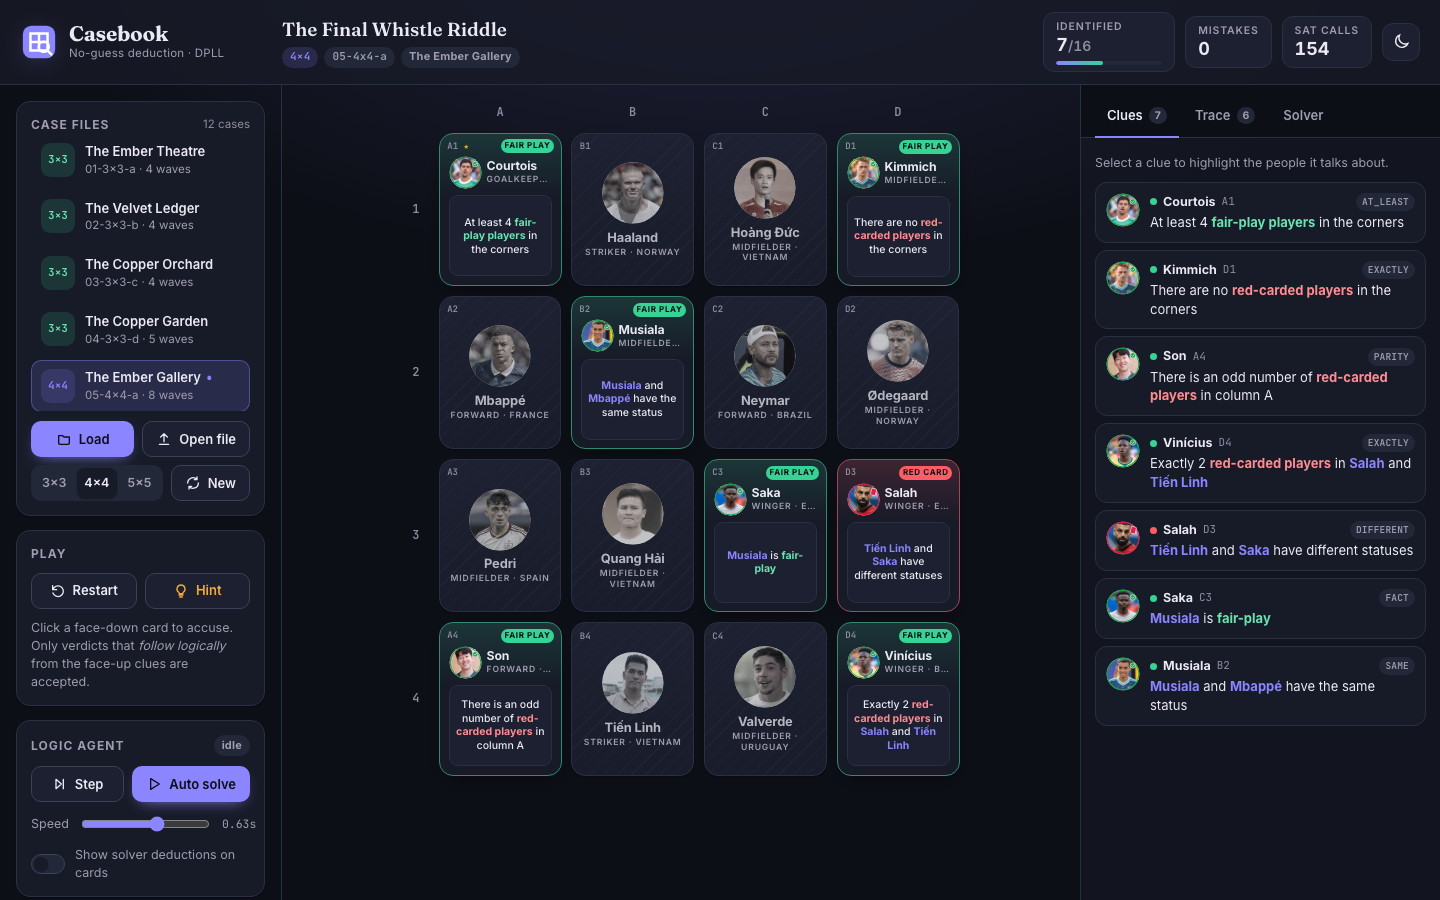
\includegraphics[width=0.88\linewidth]{gui_play.png}
\caption{Đang chơi câu đố $4\times4$: thẻ đã lật, danh sách manh mối và trace của agent.}
\end{figure}

\begin{figure}[H]
\centering
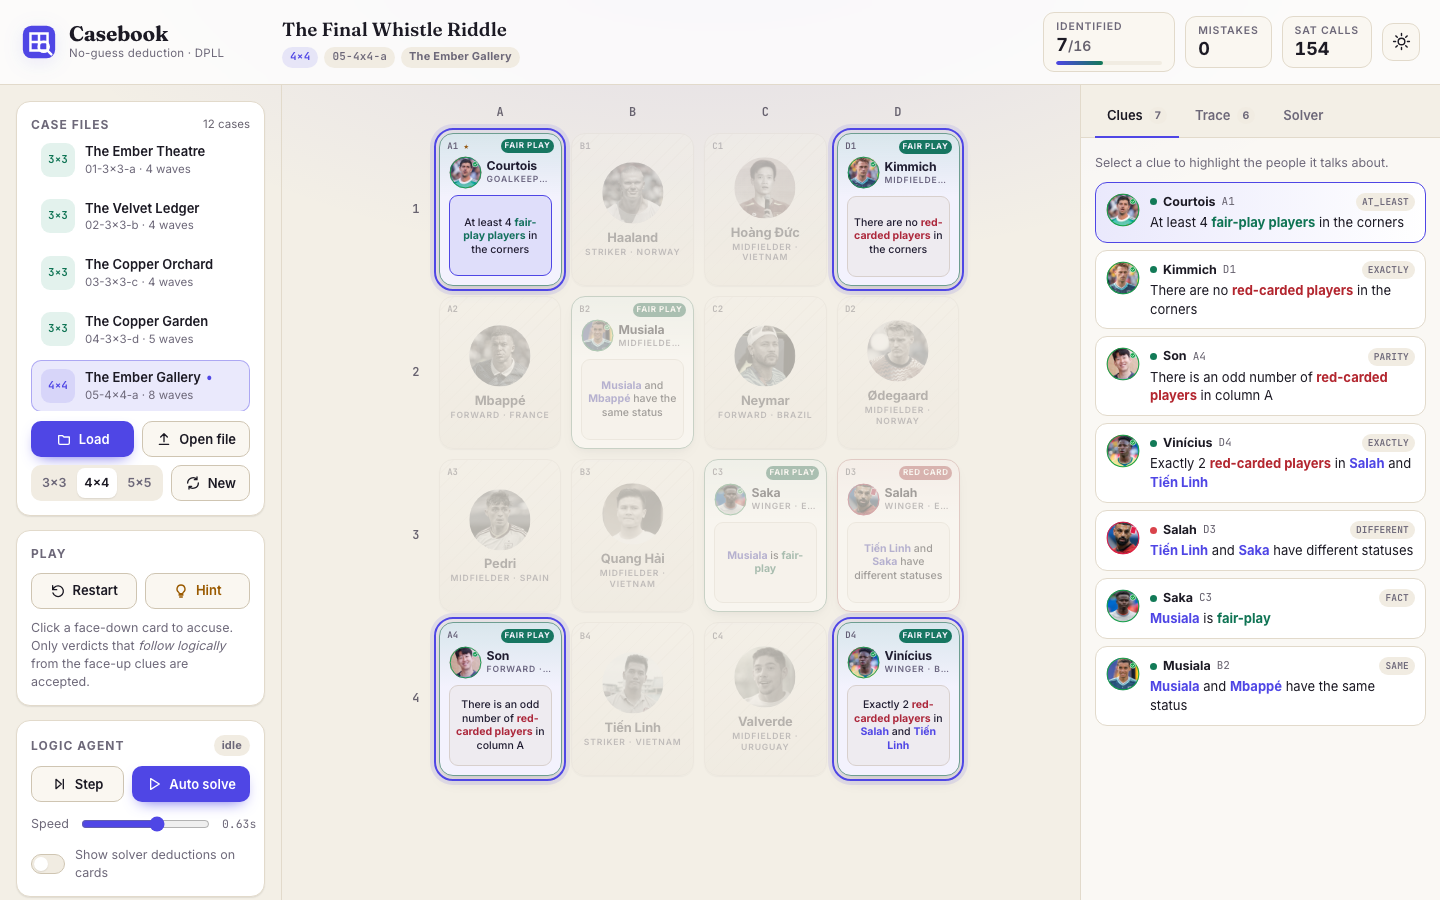
\includegraphics[width=0.88\linewidth]{gui_select.png}
\caption{Chọn một manh mối: ô được đếm (viền liền) và người được nhắc tên (viền đứt) được làm nổi bật.}
\end{figure}

\subsection{Bộ nhân vật cầu thủ}
Thay cho nhân vật thám tử lưu trong file câu đố, giao diện mặc định hiển thị 30 cầu thủ nổi tiếng (Messi, Ronaldo, Mbappé, Haaland, Modrić, \dots) và các tuyển thủ Việt Nam (Quang Hải, Văn Hậu, Tiến Linh, Hoàng Đức), mỗi người kèm vị trí và đội tuyển (giữ bằng tiếng Anh như trong giao diện, ví dụ ``Forward · Argentina''). Hai trạng thái được gọi theo ngôn ngữ bóng đá: \textbf{Red card} (thay cho Criminal) và \textbf{Fair play} (thay cho Innocent) trên nhãn thẻ, nút phán đoán, manh mối (ví dụ ``Exactly 1 red-carded player in row 2''), thông báo và trace; logic bên dưới vẫn chỉ là $C_i$ đúng/sai.

\textbf{Ảnh chân dung.} Mỗi cầu thủ dùng một ảnh thật từ Wikimedia Commons với giấy phép tự do (CC BY, CC BY-SA, public domain), được cắt vuông $320\times320$ quanh khuôn mặt bằng bộ phát hiện khuôn mặt Vision của macOS (thư mục \code{Source/web/portraits/}); tác giả và giấy phép của từng ảnh được ghi trong \code{Source/web/portraits/CREDITS.md}. Nếu thiếu file ảnh, chương trình vẽ một avatar SVG mặc áo đấu đội tuyển (với sự hỗ trợ của trợ lý AI, xem Phụ lục). Vai trong trò chơi là trạng thái ngẫu nhiên, không mang hàm ý gì về người thật (giao diện cũng hiển thị lưu ý này).

Bộ cầu thủ \textbf{chỉ mang tính hiển thị}: nó thay tên, nghề, ảnh và cách gọi trạng thái nhưng giữ nguyên ô, manh mối và lời giải; tên được xếp theo bảng chữ cái theo hàng (không phân biệt dấu). Với lưới lớn hơn 30 ô (file tự tải lên), chương trình giữ tên nhân vật trong file. Kiểm thử xác nhận agent cho cùng một chuỗi phán đoán với tên gốc và tên cầu thủ.

\begin{figure}[H]
\centering
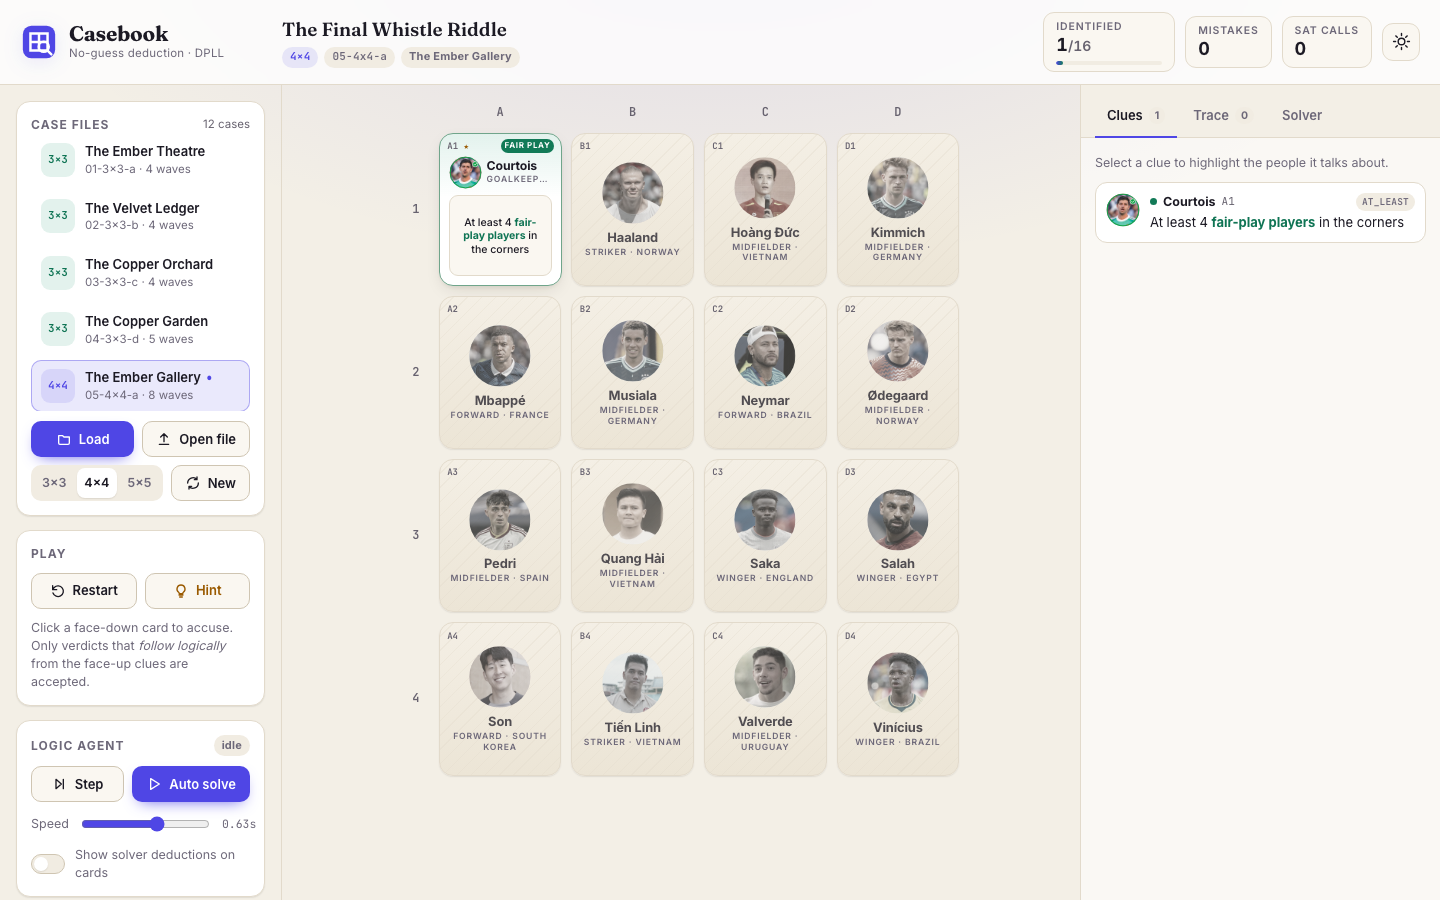
\includegraphics[width=0.88\linewidth]{gui_football.png}
\caption{Câu đố $4\times4$ với bộ cầu thủ: thẻ ``Fair play'' đã lật và manh mối dùng cách gọi bóng đá.}
\end{figure}

% =========================================================================
% CHƯƠNG 6: KẾT QUẢ THỰC NGHIỆM & ĐÁNH GIÁ
% =========================================================================
\section{Kết quả thực nghiệm \& Đánh giá}

\subsection{Cấu hình thực nghiệm}
Thực nghiệm chạy trên MacBook Pro Apple M1 Pro (16 GB RAM), macOS 26.6, Python 3.14.6. Bộ dữ liệu gồm 12 câu đố: 4 câu $3\times3$, 4 câu $4\times4$, 2 câu $5\times5$ (ca ép tải) do bộ sinh tạo với seed cố định, và 2 ca lỗi viết tay: \code{90-3x3-ambiguous} (nhiều nghiệm, kỳ vọng STUCK) và \code{91-3x3-inconsistent} (manh mối mâu thuẫn, kỳ vọng INCONSISTENT). Mỗi câu đố chạy với 3 cấu hình: \code{filter+auto} (mặc định), \code{naive+auto} và \code{filter+counter}, tổng cộng 36 lượt. Số liệu được sinh bởi \code{python3 experiments.py} (lưu ở \code{Source/results/}); bảng và biểu đồ dưới đây được tạo trực tiếp từ file kết quả đó. Mỗi lần gọi SAT có giới hạn 30 giây; không lượt nào bị timeout. Cột ``ms'' là thời gian thực của cả vòng suy diễn, gồm cả việc engine kiểm tra lại từng phán đoán (thời gian SAT riêng của agent chiếm khoảng 36\% con số này). Thời gian có thể dao động nhẹ giữa các lần chạy.

\begin{table}[H]\centering\scriptsize\setlength{\tabcolsep}{3pt}
\resizebox{\textwidth}{!}{%
\begin{tabular}{lcrrrrrrrrrrl}\toprule
Puzzle & Kết quả & Biến chính & Biến phụ & Mệnh đề & SAT & Quyết định & Lan truyền & Quay lui & Bước & Wave & ms & Duy nhất\\\midrule
\texttt{01-3x3-a} & \textcolor{solved}{\textbf{\scriptsize SOLVED}} & 9 & 0 & 32 & 42 & 4 & 215 & 0 & 8 & 4 & 1.8 & \scriptsize UNIQUE\\
\texttt{02-3x3-b} & \textcolor{solved}{\textbf{\scriptsize SOLVED}} & 9 & 1 & 45 & 40 & 14 & 212 & 1 & 8 & 4 & 1.9 & \scriptsize UNIQUE\\
\texttt{03-3x3-c} & \textcolor{solved}{\textbf{\scriptsize SOLVED}} & 9 & 51 & 189 & 43 & 47 & 1\,196 & 0 & 8 & 4 & 7.4 & \scriptsize UNIQUE\\
\texttt{04-3x3-d} & \textcolor{solved}{\textbf{\scriptsize SOLVED}} & 9 & 3 & 39 & 41 & 10 & 249 & 0 & 8 & 5 & 1.8 & \scriptsize UNIQUE\\
\texttt{05-4x4-a} & \textcolor{solved}{\textbf{\scriptsize SOLVED}} & 16 & 24 & 270 & 131 & 35 & 1\,460 & 0 & 15 & 8 & 11.9 & \scriptsize UNIQUE\\
\texttt{06-4x4-b} & \textcolor{solved}{\textbf{\scriptsize SOLVED}} & 16 & 14 & 152 & 127 & 49 & 1\,676 & 2 & 15 & 6 & 10.1 & \scriptsize UNIQUE\\
\texttt{07-4x4-c} & \textcolor{solved}{\textbf{\scriptsize SOLVED}} & 16 & 4 & 206 & 124 & 135 & 1\,214 & 28 & 15 & 6 & 15.3 & \scriptsize UNIQUE\\
\texttt{08-4x4-d} & \textcolor{solved}{\textbf{\scriptsize SOLVED}} & 16 & 181 & 628 & 122 & 79 & 3\,333 & 11 & 15 & 6 & 18.3 & \scriptsize UNIQUE\\
\texttt{09-5x5-a} & \textcolor{solved}{\textbf{\scriptsize SOLVED}} & 25 & 156 & 785 & 298 & 712 & 11\,855 & 6 & 24 & 7 & 135.7 & \scriptsize UNIQUE\\
\texttt{10-5x5-b} & \textcolor{solved}{\textbf{\scriptsize SOLVED}} & 25 & 487 & 1\,626 & 315 & 259 & 64\,527 & 0 & 24 & 12 & 311.5 & \scriptsize UNIQUE\\
\texttt{90-3x3-amb} & \textcolor{stuck}{\textbf{\scriptsize STUCK}} & 9 & 0 & 5 & 8 & 7 & 23 & 0 & 0 & 0 & 0.1 & \scriptsize MULTIPLE\\
\texttt{91-3x3-inc} & \textcolor{incons}{\textbf{\scriptsize INCONSISTENT}} & 9 & 0 & 6 & 10 & 0 & 29 & 0 & 1 & 1 & 0.2 & \scriptsize NO\_SOLUTION\\
\bottomrule\end{tabular}}
\caption{Kết quả với cấu hình mặc định (\texttt{filter} + \texttt{auto}). ``Biến chính/phụ'' và ``Mệnh đề'' là kích thước $\KB_t$ lớn nhất trong lượt giải; ``SAT'' là tổng số lần gọi DPLL của agent; ``ms'' là thời gian thực của cả vòng suy diễn (gồm cả việc engine kiểm tra lại từng phán đoán).}
\label{tab:main}
\end{table}

\begin{table}[H]\centering\scriptsize\setlength{\tabcolsep}{3.5pt}
\resizebox{\textwidth}{!}{%
\begin{tabular}{l rr rr | rr rr rr}\toprule
 & \multicolumn{2}{c}{Số lần gọi SAT} & \multicolumn{2}{c|}{Thời gian (ms)} & \multicolumn{2}{c}{Biến phụ} & \multicolumn{2}{c}{Mệnh đề} & \multicolumn{2}{c}{Lan truyền}\\
Puzzle & naive & filter & naive & filter & auto & counter & auto & counter & auto & counter\\\midrule
\texttt{01-3x3-a} & 80 & 42 & 2.2 & 1.8 & 0 & 27 & 32 & 102 & 215 & 767\\
\texttt{02-3x3-b} & 80 & 40 & 2.7 & 1.9 & 1 & 59 & 45 & 198 & 212 & 1\,005\\
\texttt{03-3x3-c} & 80 & 43 & 12.3 & 7.4 & 51 & 57 & 189 & 205 & 1\,196 & 1\,418\\
\texttt{04-3x3-d} & 80 & 41 & 2.4 & 1.8 & 3 & 30 & 39 & 112 & 249 & 735\\
\texttt{05-4x4-a} & 255 & 131 & 18.1 & 11.9 & 24 & 205 & 270 & 665 & 1\,460 & 6\,487\\
\texttt{06-4x4-b} & 255 & 127 & 17.4 & 10.1 & 14 & 160 & 152 & 536 & 1\,676 & 7\,080\\
\texttt{07-4x4-c} & 255 & 124 & 27.7 & 15.3 & 4 & 189 & 206 & 612 & 1\,214 & 8\,945\\
\texttt{08-4x4-d} & 255 & 122 & 32.5 & 18.3 & 181 & 238 & 628 & 782 & 3\,333 & 5\,400\\
\texttt{09-5x5-a} & 624 & 298 & 290.1 & 135.7 & 156 & 465 & 785 & 1\,471 & 11\,855 & 57\,034\\
\texttt{10-5x5-b} & 624 & 315 & 634.7 & 311.5 & 487 & 644 & 1\,626 & 2\,013 & 64\,527 & 67\,941\\
\texttt{90-3x3-amb} & 17 & 8 & 0.1 & 0.1 & 0 & 7 & 5 & 24 & 23 & 79\\
\texttt{91-3x3-inc} & 18 & 10 & 0.2 & 0.2 & 0 & 2 & 6 & 10 & 29 & 49\\
\bottomrule\end{tabular}}
\caption{So sánh chiến lược truy vấn (\texttt{naive} và \texttt{filter}, cùng mã hóa \texttt{auto}) và cách mã hóa ràng buộc đếm (\texttt{auto} và \texttt{counter}, cùng chiến lược \texttt{filter}).}
\label{tab:compare}
\end{table}

\begin{figure}[H]
\centering
\begin{tikzpicture}\begin{axis}[width=0.94\linewidth,height=5.2cm,ybar,/pgf/number format/1000 sep={\,},bar width=4pt,symbolic x coords={01,02,03,04,05,06,07,08,09,10,90,91},xtick=data,ymin=0,ylabel={Số lần gọi SAT},title={\small Số lần gọi SAT của agent theo chiến lược},legend style={at={(0.02,0.98)},anchor=north west,font=\scriptsize,draw=none,fill=white,fill opacity=.8,text opacity=1},tick label style={font=\scriptsize},label style={font=\footnotesize},enlarge x limits=0.05,ymajorgrids,grid style={gray!25}]
\addplot[fill=naivec,draw=none] coordinates {(01,80) (02,80) (03,80) (04,80) (05,255) (06,255) (07,255) (08,255) (09,624) (10,624) (90,17) (91,18)};
\addplot[fill=filterc,draw=none] coordinates {(01,42) (02,40) (03,43) (04,41) (05,131) (06,127) (07,124) (08,122) (09,298) (10,315) (90,8) (91,10)};
\legend{naive,filter}
\end{axis}\end{tikzpicture}
\caption{Chiến lược lọc mô hình giảm khoảng một nửa số lần gọi SAT (nhãn trục ngang là mã câu đố).}
\end{figure}

\begin{figure}[H]
\centering
\begin{tikzpicture}\begin{axis}[width=0.94\linewidth,height=5.2cm,ybar,/pgf/number format/1000 sep={\,},bar width=4pt,symbolic x coords={01,02,03,04,05,06,07,08,09,10,90,91},xtick=data,ymin=0,ylabel={mệnh đề},title={\small Số mệnh đề của $\KB_t$ lớn nhất theo cách mã hóa},legend style={at={(0.02,0.98)},anchor=north west,font=\scriptsize,draw=none,fill=white,fill opacity=.8,text opacity=1},tick label style={font=\scriptsize},label style={font=\footnotesize},enlarge x limits=0.05,ymajorgrids,grid style={gray!25}]
\addplot[fill=filterc,draw=none] coordinates {(01,32) (02,45) (03,189) (04,39) (05,270) (06,152) (07,206) (08,628) (09,785) (10,1626) (90,5) (91,6)};
\addplot[fill=counterc,draw=none] coordinates {(01,102) (02,198) (03,205) (04,112) (05,665) (06,536) (07,612) (08,782) (09,1471) (10,2013) (90,24) (91,10)};
\legend{auto (trực tiếp khi nhỏ),counter}
\end{axis}\end{tikzpicture}
\caption{Số mệnh đề: chế độ \code{auto} (trực tiếp khi nhỏ) so với \code{counter} (luôn dùng bộ đếm).}
\end{figure}

\begin{figure}[H]
\centering
\begin{tikzpicture}\begin{semilogyaxis}[log origin=infty,width=0.94\linewidth,height=5.2cm,ybar,/pgf/number format/1000 sep={\,},bar width=4pt,symbolic x coords={01,02,03,04,05,06,07,08,09,10,90,91},xtick=data,ymin=0.01,ylabel={ms},title={\small Tổng thời gian giải (thang log)},legend style={at={(0.02,0.98)},anchor=north west,font=\scriptsize,draw=none,fill=white,fill opacity=.8,text opacity=1},tick label style={font=\scriptsize},label style={font=\footnotesize},enlarge x limits=0.05,ymajorgrids,grid style={gray!25}]
\addplot[fill=filterc,draw=none] coordinates {(01,1.8) (02,1.9) (03,7.4) (04,1.8) (05,11.9) (06,10.1) (07,15.3) (08,18.3) (09,135.7) (10,311.5) (90,0.1) (91,0.2)};
\addplot[fill=naivec,draw=none] coordinates {(01,2.2) (02,2.7) (03,12.3) (04,2.4) (05,18.1) (06,17.4) (07,27.7) (08,32.5) (09,290.1) (10,634.7) (90,0.1) (91,0.2)};
\addplot[fill=counterc,draw=none] coordinates {(01,3.5) (02,5.2) (03,8.3) (04,3.6) (05,25.0) (06,26.1) (07,39.1) (08,24.0) (09,291.6) (10,321.7) (90,0.2) (91,0.2)};
\legend{filter+auto,naive+auto,filter+counter}
\end{semilogyaxis}\end{tikzpicture}
\caption{Tổng thời gian giải mỗi câu đố theo 3 cấu hình (thang logarit).}
\end{figure}

\subsection{Đánh giá}
\begin{itemize}[noitemsep]
    \item \textbf{Đúng đắn:} cả 36 lượt đều cho đúng kết quả kỳ vọng (0 lượt sai lệch). Mọi câu đố hợp lệ được giải hết không cần đoán và đều \code{UNIQUE}; ca nhiều nghiệm dừng ở \code{STUCK} (agent từ chối đoán), ca mâu thuẫn được phát hiện là \code{INCONSISTENT} ngay khi $\KB$ trở thành UNSAT.
    \item \textbf{Lọc mô hình:} trên 10 câu đố hợp lệ, \code{filter} dùng 1\,283 lần gọi SAT so với 2\,588 của \code{naive} (giảm 50.4\%), với cùng kết quả phân loại.
    \item \textbf{Cách mã hóa:} chế độ \code{counter} sinh nhiều mệnh đề hơn \code{auto} từ 1.1 đến 4.4 lần trên 10 câu đố hợp lệ (phần lớn ràng buộc đếm có vùng nhỏ nên tổ hợp trực tiếp ít mệnh đề hơn) và tốn nhiều lượt lan truyền hơn. Ưu điểm của bộ đếm là tăng trưởng đa thức $O(n\cdot k)$; chế độ \code{auto} dùng mã hóa trực tiếp khi nó sinh không quá 300 mệnh đề và chuyển sang bộ đếm khi vượt ngưỡng (xét riêng từng nửa $\ge$/$\le$), trong bộ dữ liệu chỉ một manh mối (\code{EXACTLY} trên 16 ô của câu \code{10}) vượt ngưỡng; biến phụ của chế độ \code{auto} ở các câu khác (ví dụ \code{03}, \code{08}) đến từ \code{COMPARE} (luôn dùng bộ đếm) và chuỗi XOR của \code{PARITY}.
    \item \textbf{Hiệu năng:} lượt chậm nhất ở cấu hình mặc định là \code{10-5x5-b} với 311.5 ms; số lần quay lui nhỏ (tối đa 28) vì mỗi phán đoán đã chứng minh trở thành mệnh đề đơn vị, giúp lan truyền đơn vị tìm ra mâu thuẫn ngay.
\end{itemize}

% =========================================================================
% CHƯƠNG 7: KIỂM THỬ & KIỂM CHỨNG
% =========================================================================
\section{Kiểm thử \& Kiểm chứng}\label{sec:test}
Bộ kiểm thử gồm 43 test (\code{python3 -m unittest discover -s tests -v} trong \code{Source/}):
\begin{itemize}[noitemsep]
    \item \textbf{Bộ mã hóa và bộ đánh giá (vét cạn):} với mọi loại manh mối (riêng ràng buộc đếm: $k = 0..8$ trên vùng lân cận của B2, đếm cả criminal và innocent) và cả 3 chế độ mã hóa, kiểm tra trên \textit{mọi} $2^9$ phép gán của lưới $3\times3$ rằng $\text{CNF} \land \text{phép gán}$ SAT $\iff$ bộ đánh giá trả True.
    \item \textbf{DPLL và vét cạn:} hàng trăm CNF ngẫu nhiên (có/không literal thuần, có assumption); mô hình trả về luôn được kiểm tra lại.
    \item \textbf{filter = naive:} trên nhiều trạng thái ngẫu nhiên, hai chiến lược cho cùng phân loại và filter không bao giờ tốn nhiều truy vấn hơn.
    \item \textbf{Engine, agent, Hint:} phân biệt đúng NOT\_PROVABLE/CONTRADICTED, phán đoán bị từ chối không đổi $\KB$, CONTRADICTED kết thúc ván cho tới khi Restart; tập manh mối của Hint đủ và tối thiểu; câu đố đi kèm đạt đúng kết quả kỳ vọng.
    \item \textbf{Máy chủ:} yêu cầu sai định dạng trả lỗi 4xx; không có phản hồi nào chứa trạng thái ẩn hay manh mối chưa lật; nước đi gửi trước khi Restart bị từ chối; sau \textit{game over} mọi gợi ý và bước của agent bị từ chối.
    \item \textbf{Bộ cầu thủ:} đủ 30 người cho lưới $5\times5$, tên và ảnh không trùng, lưới lớn hơn giữ tên trong file, agent cho cùng kết quả với tên gốc và tên cầu thủ.
\end{itemize}
Ngoài ra mã nguồn được review độc lập nhiều vòng (lõi logic, máy chủ/giao diện, báo cáo) bằng các kiểm tra ngẫu nhiên quy mô lớn (hàng nghìn cặp manh mối--chế độ mã hóa, hàng nghìn CNF ngẫu nhiên); các lỗi tìm được đều đã sửa và được phủ bởi test hồi quy.

% =========================================================================
% CHƯƠNG 8: HẠN CHẾ & HƯỚNG PHÁT TRIỂN
% =========================================================================
\section{Hạn chế \& Hướng phát triển}
\begin{itemize}[noitemsep]
    \item DPLL quay lui theo thời gian, chưa có học mệnh đề (CDCL) hay heuristic chọn biến động; đủ nhanh cho lưới đến $5\times5$ nhưng sẽ chậm với lưới lớn hơn.
    \item Mỗi bước, agent phân loại lại toàn bộ $\KB_t$ từ đầu; có thể giải tăng dần (giữ trạng thái solver giữa các bước).
    \item \code{EXACTLY} ở chế độ counter dựng hai bộ đếm riêng; dùng chung một bộ đếm sẽ giảm khoảng một nửa biến phụ. Có thể bổ sung mã hóa mạng sắp xếp (sorting network) cho vùng rất lớn.
    \item Sinh câu đố $5\times5$ thường mất từ 1 đến 13 giây (có khi lâu hơn) vì phải mô phỏng người chơi không đoán nhiều lần.
\end{itemize}

% =========================================================================
% CHƯƠNG 9: THAM KHẢO & PHỤ LỤC
% =========================================================================
\section{Tham khảo \& Phụ lục}

\subsection{Tài liệu tham khảo}
\begin{enumerate}[noitemsep]
    \item Stuart Russell and Peter Norvig. \textit{Artificial Intelligence: A Modern Approach (4th Edition)}. Pearson, 2020. (Chương 7: Logical Agents).
    \item Martin Davis, George Logemann, and Donald Loveland. \textit{A Machine Program for Theorem-Proving}. Communications of the ACM, 5(7):394--397, 1962.
    \item G. S. Tseitin. \textit{On the Complexity of Derivation in Propositional Calculus}. Studies in Constructive Mathematics and Mathematical Logic, Part II, 1968 (in lại trong \textit{Automation of Reasoning 2}, Springer, 1983, tr. 466--483).
    \item Carsten Sinz. \textit{Towards an Optimal CNF Encoding of Boolean Cardinality Constraints}. CP 2005, LNCS 3709.
    \item A. Biere, M. Heule, H. van Maaren, T. Walsh (eds.). \textit{Handbook of Satisfiability}. IOS Press, 2021.
    \item Martin Davis and Hilary Putnam. \textit{A Computing Procedure for Quantification Theory}. Journal of the ACM, 7(3):201--215, 1960.
    \item Đề bài CSC14003 Project 2 (Griductive Solver) và trang hướng dẫn luật chơi Griductive.
    \item Tài liệu Python: \code{http.server}, \code{dataclasses}, \code{unittest} (docs.python.org).
\end{enumerate}

\subsection{Ứng dụng Generative AI}
Trong quá trình thực hiện, nhóm sử dụng trợ lý lập trình \textbf{Claude Code (Anthropic)} để hỗ trợ viết mã nguồn, bộ kiểm thử, bộ câu đố, giao diện và bản nháp báo cáo; các thành viên đã đọc, chạy, kiểm tra lại và chịu trách nhiệm về toàn bộ nội dung nộp. Một số prompt tiêu biểu:
\begin{itemize}[noitemsep]
    \item \textit{``Giải thích cho tôi các khái niệm CNF, SAT, DPLL.''}
    \item \textit{``Thực hiện toàn bộ đồ án đến khi hoàn thành, UI/UX càng đẹp càng tốt, nhớ review nghiêm ngặt nhiều vòng để tránh lỗi.''}
    \item \textit{``Tiến hành kiểm tra lại toàn bộ project, tìm các chỗ chưa hoàn thiện hoặc bị lỗi rồi sửa lại.''}
    \item \textit{``Thêm các chủ đề nhân vật vào trò chơi, ví dụ cầu thủ bóng đá hoặc nhân vật anime, tự tạo avatar cho từng nhân vật.''}
    \item \textit{``Tốt hơn là hãy sử dụng các cầu thủ và nhân vật anime có thật.''}
    \item \textit{``Lên mạng lấy các tấm hình của mỗi nhân vật rồi cắt ra; trong bóng đá thay tội phạm bằng bị thẻ đỏ.''}
    \item \textit{``Không có hình thì bỏ luôn đi.''}
    \item \textit{``Bỏ anime đi, dùng cầu thủ làm mặc định, bỏ classic luôn.''}
    \item \textit{``Khi chọn sai verdict của 1 player thì game over luôn thay vì báo là contradict.''}
    \item \textit{``Tinh chỉnh báo cáo cho chính xác theo mã nguồn hiện tại.''}
\end{itemize}

\subsection{Kho lưu trữ mã nguồn \& Video minh họa}
\begin{itemize}
    \item \textbf{Kho lưu trữ mã nguồn (GitHub Repository):} \\
    \url{https://github.com/LGKAI/Griductive-Solver}

    \item \textbf{Video minh họa sản phẩm (Video Demo):} \\
    \textcolor{red}{[Dán link Google Drive của video demo, quyền ``Anyone with the link]}
\end{itemize}

\subsection{Cách chạy chương trình}
\begin{Verbatim}[fontsize=\small]
cd Source
python3 main.py                                  # giao diện web
python3 main.py --solve puzzles/05-4x4-a.json -v # in trace
python3 main.py --check puzzles/05-4x4-a.json    # nghiệm duy nhất
python3 experiments.py                           # chạy thực nghiệm
python3 -m unittest discover -s tests -v         # bộ kiểm thử
\end{Verbatim}

\end{document}